\documentclass{article}
% translate with >> pdflatex -shell-escape <file>

% This file is an extract of the PGFPLOTS manual, copyright by Christian Feuersaenger.
% 
% Feel free to use it as long as you cite the pgfplots manual properly.
%
% See
%   http://pgfplots.sourceforge.net/pgfplots.pdf
% for the complete manual.
%
% Any required input files (for <plot table> or <plot file> or the table package) can be downloaded
% at
% http://www.ctan.org/tex-archive/graphics/pgf/contrib/pgfplots/doc/latex/
% and
% http://www.ctan.org/tex-archive/graphics/pgf/contrib/pgfplots/doc/latex/plotdata/

\usepackage{pgfplots}
\pgfplotsset{compat=newest}

\pagestyle{empty}
\usepackage{pgfplotstable}

\begin{document}
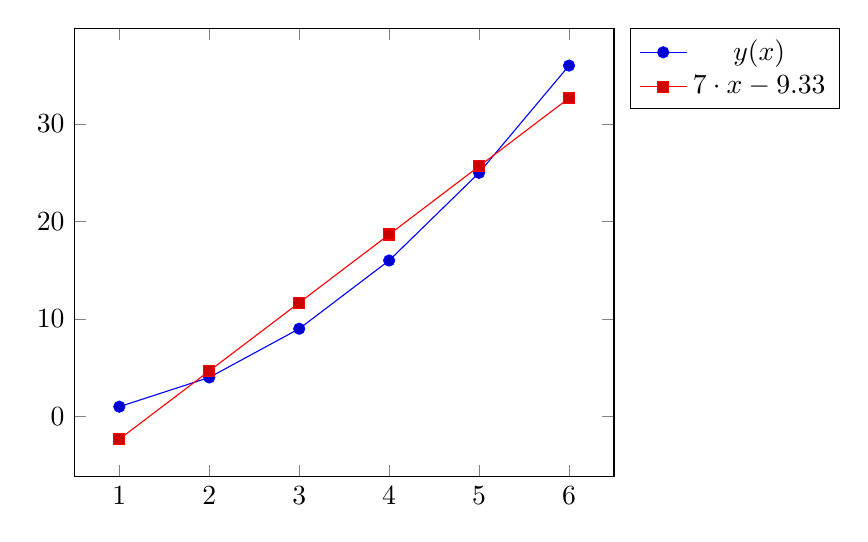
\begin{tikzpicture}
	\begin{axis}[legend pos=outer north east]
	\addplot table {% plot X versus Y. This is original data.
		X Y
		1 1 
		2 4
		3 9
		4 16
		5 25
		6 36
	};
	\addplot table[
		y={create col/linear regression={y=Y}}] % compute a linear regression from the input table
	{
		X Y
		1 1 
		2 4
		3 9
		4 16
		5 25
		6 36
	};
	%\xdef\slope{\pgfplotstableregressiona} %<-- might be handy occasionally
	\addlegendentry{$y(x)$}
	\addlegendentry{% 
		$\pgfmathprintnumber{\pgfplotstableregressiona} \cdot x  
		\pgfmathprintnumber[print sign]{\pgfplotstableregressionb}$}
	\end{axis}
\end{tikzpicture}
\end{document}
